
This section contains additional graphs with data to simulation comparisons.
Figure~\ref{fig:nbtags} displays the number of events in each btag category after full
selection. Distributions of the $\pt$ after preselection cuts are given in
Figures~\ref{fig:lepptele} and~\ref{fig:lepptmuon} for the leading and subleading lepton, 
for electrons and muons. 
In Figure~\ref{fig:jetpt} for the leading and subleading jet. In addition, the
reconstructed number of good vertices in data and in reweighed simulation is
depicted in Figure~\ref{fig:shiftedDataPileup2} for the electron and muon channels combined.

\begin{figure}[h]
\begin{center}
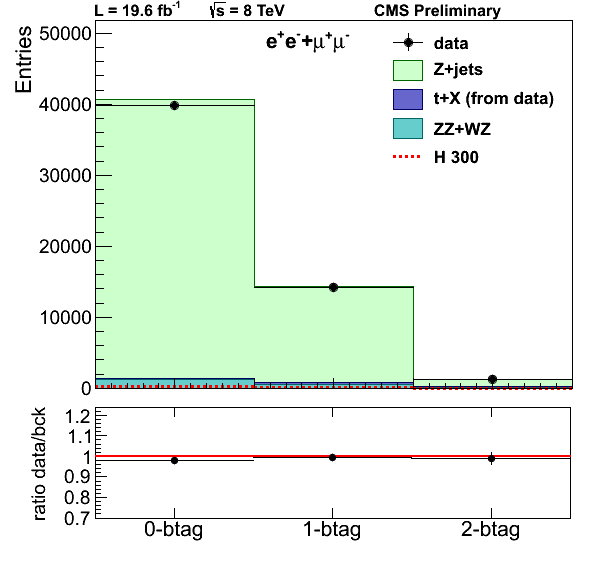
\includegraphics[width=0.49\textwidth]{plots/extra/NBTAG_ll.png}
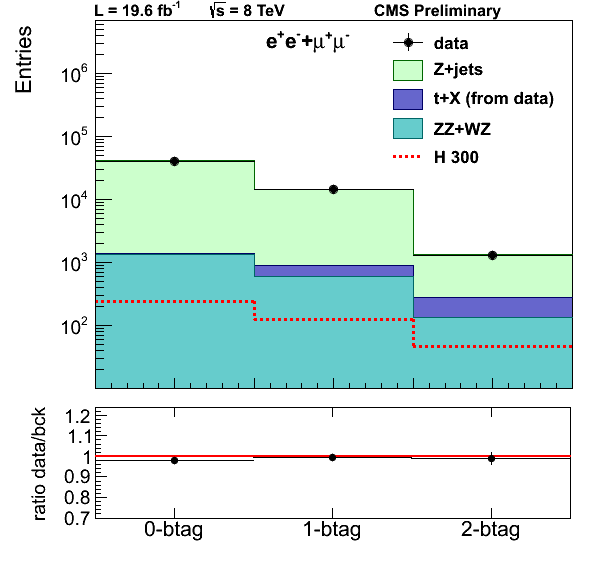
\includegraphics[width=0.49\textwidth]{plots/extra/LOGNBTAG_ll.png}
\caption{Number of events in each btag category after full
selection, for the electron and muon channel combined, in linear (left) and logarithmic scales (right).
Dots indicate data, pale green histogram corrected Z+jets simulation,
light blue simulated diboson background and dark blue $\ttbar$ events from data (which
includes single top, WW, $\Zo\to\TT$+jets).
}
\label{fig:nbtags}
\end{center}
\end{figure}

\vspace*{-5mm}
\begin{figure}[h]
\begin{center}
%% 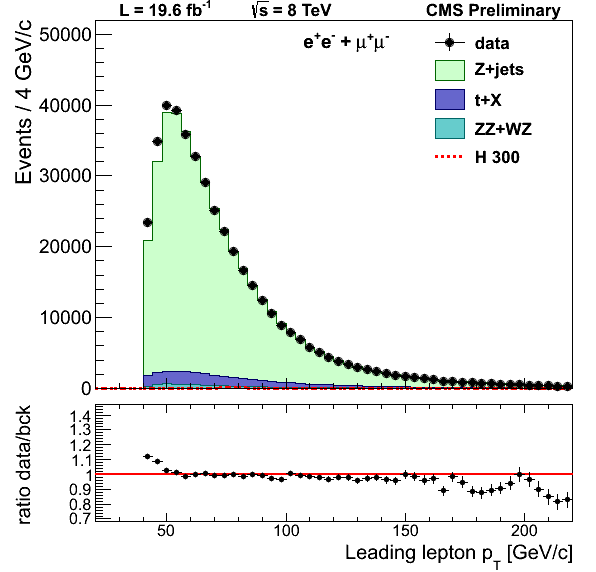
\includegraphics[width=0.32\textwidth]{plots/extra/h_ll_lep_pt0.png}
%% 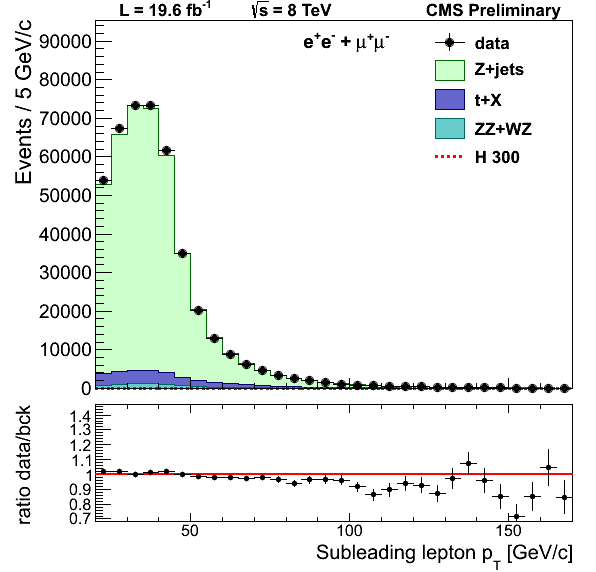
\includegraphics[width=0.32\textwidth]{plots/extra/h_ll_lep_pt1.png} \\
%% 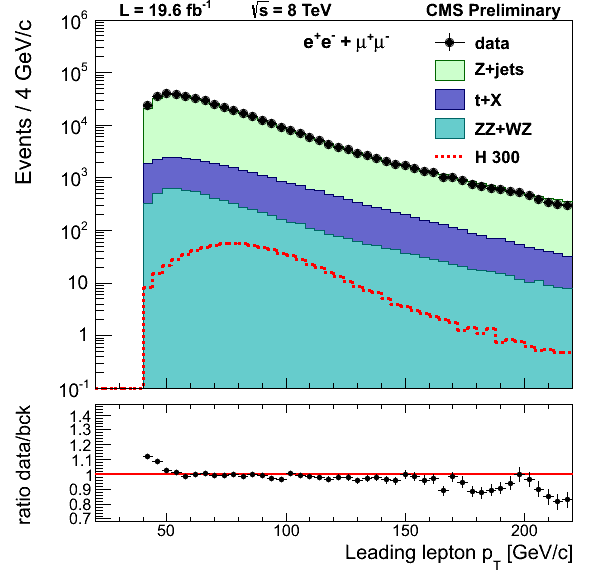
\includegraphics[width=0.32\textwidth]{plots/extra/lh_ll_lep_pt0.png}
%% 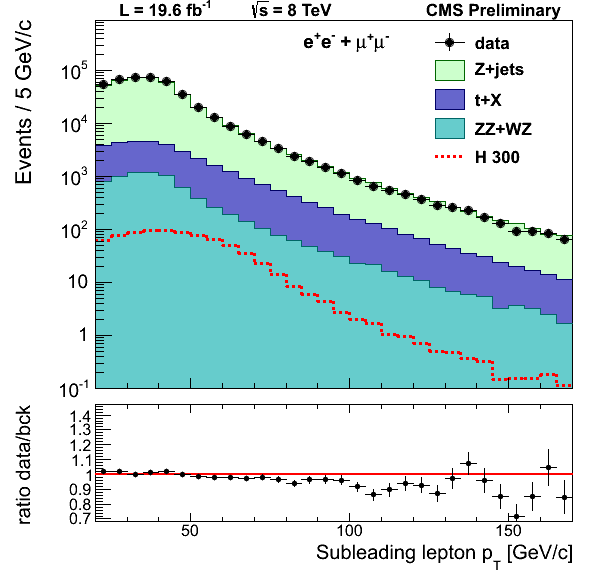
\includegraphics[width=0.32\textwidth]{plots/extra/lh_ll_lep_pt1.png}
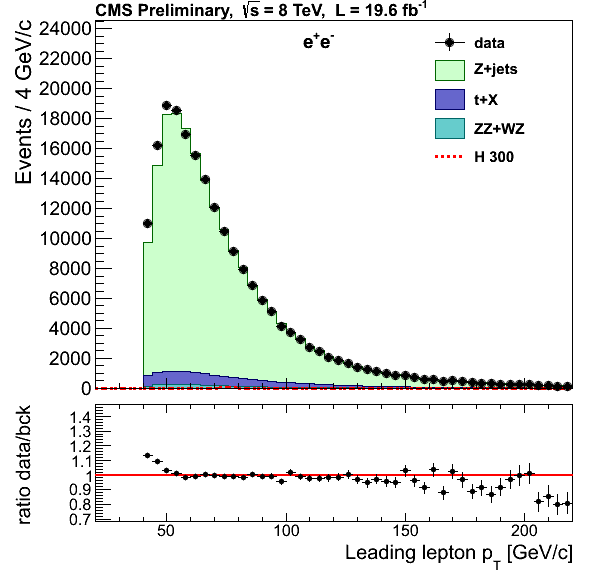
\includegraphics[width=0.32\textwidth]{plots/extra/h_ee_lep_pt0.png}
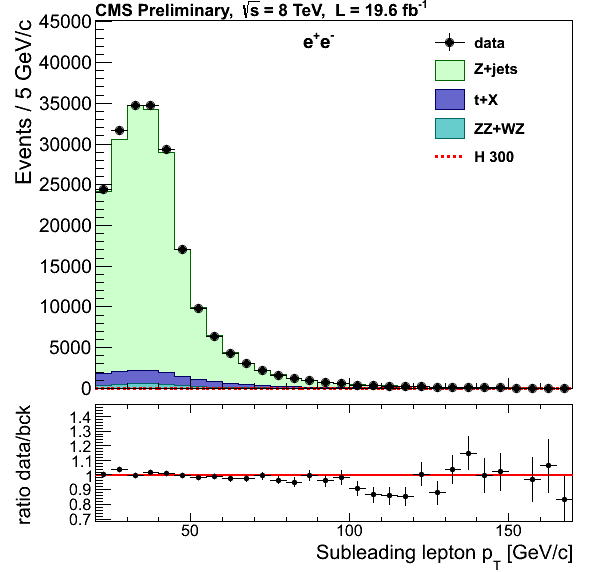
\includegraphics[width=0.32\textwidth]{plots/extra/h_ee_lep_pt1.png} \\
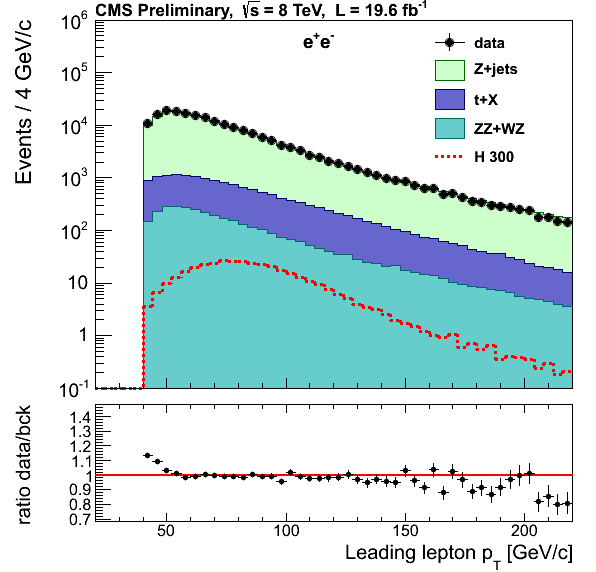
\includegraphics[width=0.32\textwidth]{plots/extra/lh_ee_lep_pt0.png}
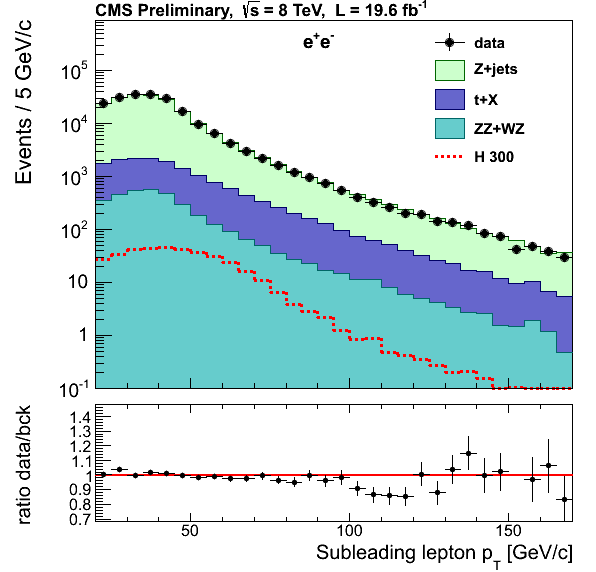
\includegraphics[width=0.32\textwidth]{plots/extra/lh_ee_lep_pt1.png}
\caption{Distributions of the $\pt$ --in linear (upper) and logarithmic scales (lower)--
of the leading (left) and subleading electron (right) after preselection cuts.
Dots indicate data, pale green histogram corrected Z+jets simulation,
light blue simulated diboson background and dark blue $\ttbar$ events from data (which
includes single top, WW, $\Zo\to\TT$+jets).
}
\label{fig:lepptele}
\end{center}
\end{figure}

\vspace*{-5mm}
\begin{figure}[h]
\begin{center}
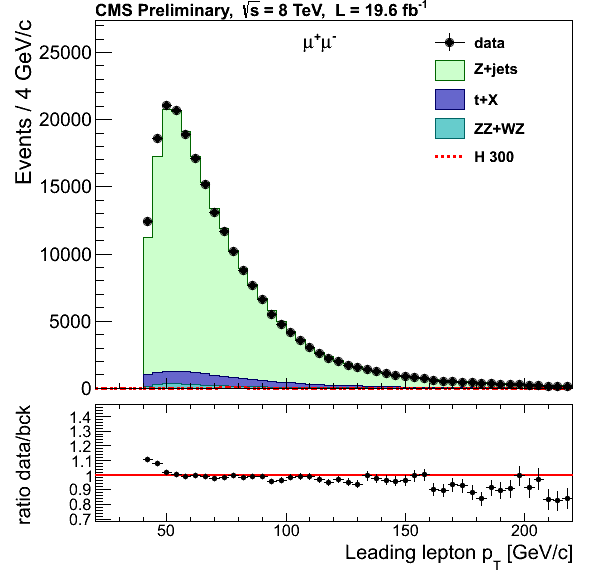
\includegraphics[width=0.32\textwidth]{plots/extra/h_mm_lep_pt0.png}
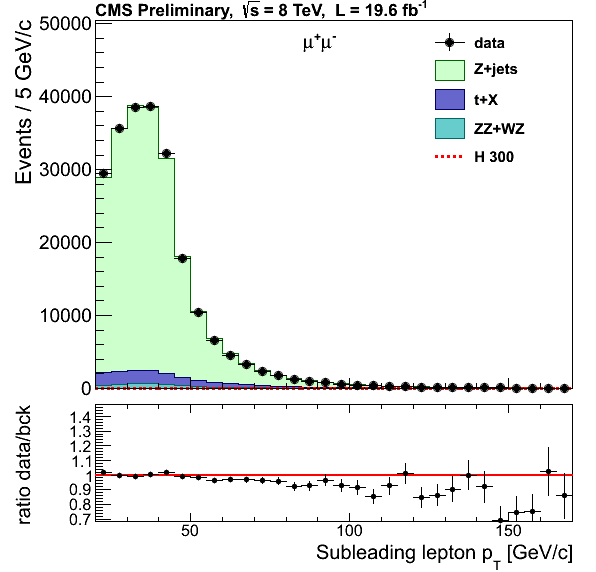
\includegraphics[width=0.32\textwidth]{plots/extra/h_mm_lep_pt1.png} \\
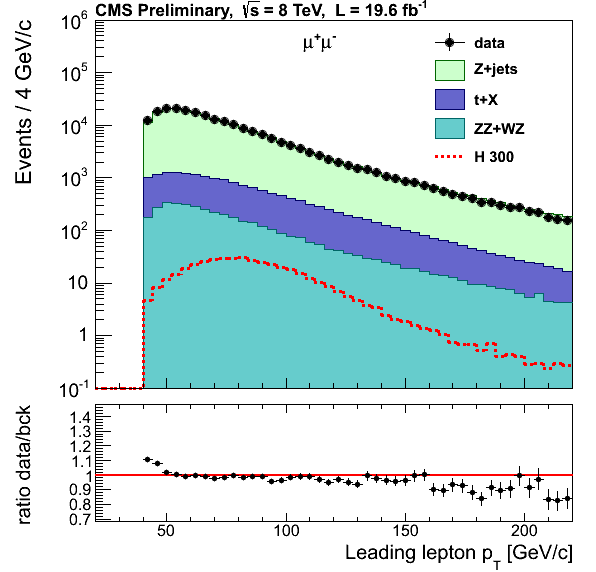
\includegraphics[width=0.32\textwidth]{plots/extra/lh_mm_lep_pt0.png}
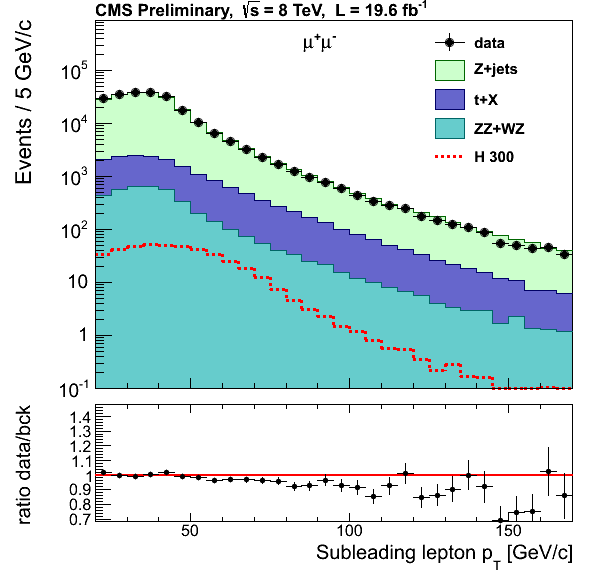
\includegraphics[width=0.32\textwidth]{plots/extra/lh_mm_lep_pt1.png}
\caption{Distributions of the $\pt$ --in linear (upper) and logarithmic scales (lower)--
of the leading (left) and subleading muon (right) after preselection cuts.
Dots indicate data, pale green histogram corrected Z+jets simulation,
light blue simulated diboson background and dark blue $\ttbar$ events from data (which
includes single top, WW, $\Zo\to\TT$+jets).
}
\label{fig:lepptmuon}
\end{center}
\end{figure}

\begin{figure}[h]
\begin{center}
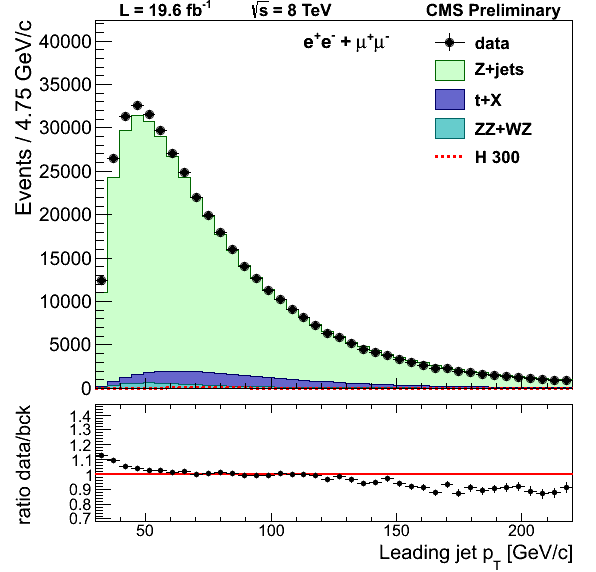
\includegraphics[width=0.32\textwidth]{plots/extra/h_ll_jet_pt0.png}
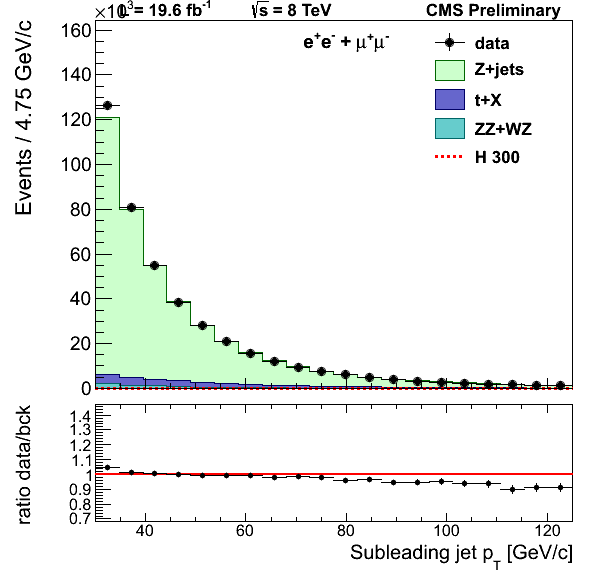
\includegraphics[width=0.32\textwidth]{plots/extra/h_ll_jet_pt1.png} \\
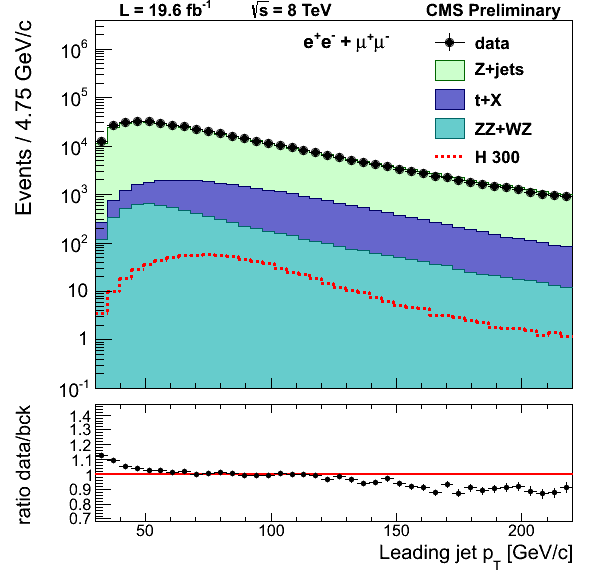
\includegraphics[width=0.32\textwidth]{plots/extra/lh_ll_jet_pt0.png}
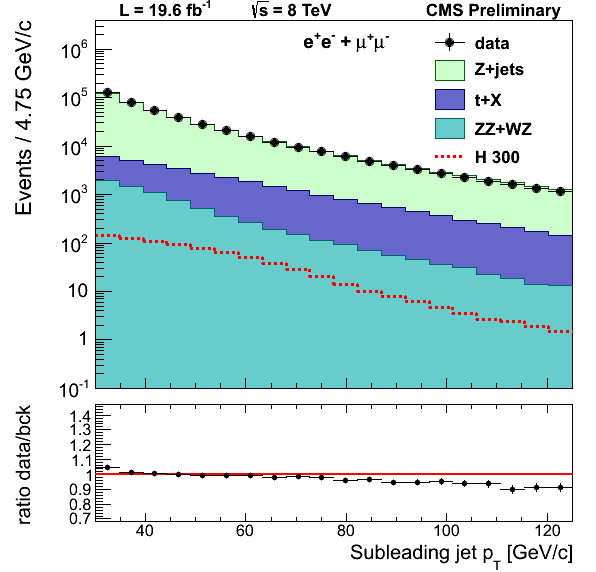
\includegraphics[width=0.32\textwidth]{plots/extra/lh_ll_jet_pt1.png}
\caption{Similar distributions for the leading (left) and subleading jet (right).}
\label{fig:jetpt}
\end{center}
\end{figure}
